\documentclass{standalone}
\begin{document}
\subsection{Prediction of Response}

The prediction of response is based on the Tumor Regression Grade (TRG) which indicates the degree of response to neoadjuvant therapy\cite{tesicoppola}. TRG ranges from 0 to 5, resulting in a different response. Lower is the TRG higher the response. 
\\
To obtain the prediction of response, a custom Support Vector Classifier (SVC) model has been implemented.
The classification is made after the standardization and PCA performed as described before.
\\
The performed steps are:

\begin{itemize}
    \item Standardization of the data
    \item PCA 
    \item Classification
\end{itemize}

Unfortunately, not for every patient, the TRG was registered in the clinical database provided by the IRCCS Sant'Orsola-Malpighi Policlinic, so patients without it were excluded from the analysis.
Moreover, since the lack of data TRG values were binarized into two main classes: 0 and 1.
Class 0 means a complete response to the neoadjuvant chemo-radiotherapy (TRG values $ \in [0, \: 1])$ while class 1 means a moderate response (TRG values $ \in [2, \: 3])$ .
In Figure \ref{classesdistrib} you can see the distribution of the two classes.

\begin{figure}[ht]

    \centering
    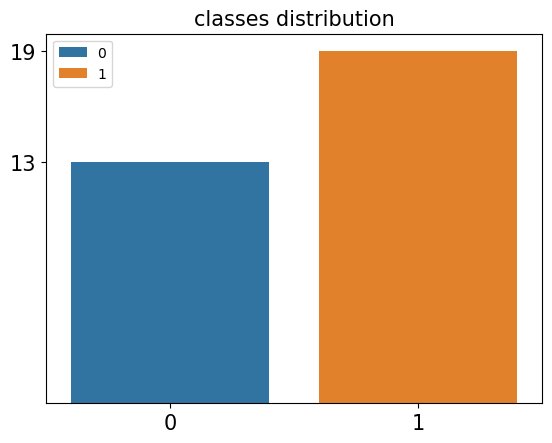
\includegraphics[width=0.52\textwidth]{../images/classesdistrib.png}

    \caption{Distribution of the classes. Class 0 means a complete response to the neo-adjuvant chemo-radiotherapy (TRG values $ \in [0, \: 1])$ while class 1 means a moderate response (TRG values $ \in [2, \: 3])$ }
    \label{classesdistrib}
    
    \end{figure}




\end{document}